\chapter{ĐO ĐẠC VÀ ĐÁNH GIÁ}

\section{Một số tập dữ liệu phổ biến được sử dụng}
\subsection{Tập dữ liệu trong không gian nhỏ}
\subsubsection*{7Scenes}
Tập dữ liệu 7-Scenes \cite{6619221} bao gồm các ảnh RGB-D thuộc bảy khung cảnh khác nhau được chụp từ một máy ảnh cầm tay Kinect RGB-D ở độ phân giải 640x480. Bảy khung cảnh bap gồm: "Chess", "Fire", "Heads", "Office", "Pumpkin", "RedKitchen" và "Stairs". Với mỗi cảnh sẽ có vài chuỗi khung ảnh RGB-D. Mỗi chuỗi bao gồm khoảng từ 1000 đến 5000 khung ảnh. Mỗi khung sẽ gồm: ảnh màu, độ sâu và vị trí.
\begin{figure}[H]
    \centering
    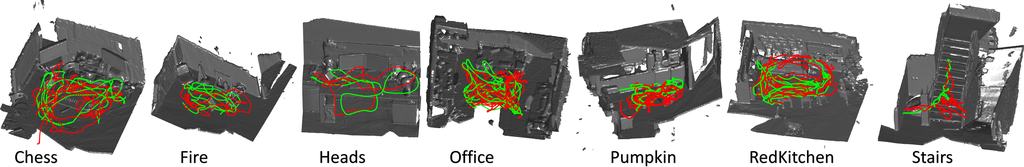
\includegraphics[width=\textwidth]{pics/Chapter2/7scenes.png}
    \caption{Minh họa tập dữ liệu 7-Scenes \cite{6619221}}
\end{figure}
\subsubsection*{Cambridge Landmark}
Tập dữ liệu Cambridge Landmarks \cite{kendall2016posenet} là một tập dữ liệu định vị thành thị bao gồm năm khung cảnh khác nhau. Các yếu tố dày đặc quan trọng như phương tiện giao thông hay người đi bộ cũng xuất hiện trong tập dữ liệu này, ngoài ra dữ liệu cũng được thu thập ở nhiều thời điểm trong ngày đại diện cho các yếu tố ánh sáng và điều kiện thời tiết khác nhau. Cambridge Landmarks được tạo ra nhờ vào việc áp dụng các kỹ thuật tái tạo kiến trúc từ chuyển động. Một chiếc điện thoại thông minh Google LG Nexus 5 được một người đi bộ trên phố sử dụng để ghi lại đoạn phim chất lượng cao cho mỗi cảnh. Mỗi đoạn phim sau đó sẽ được lấy mẫu với tần số 2Hz để trích xuất ảnh cho quy trình tái tạo kiến trúc từ chuyển động. Mỗi vị trí máy ảnh sẽ cách nhau khoảng 1m.
\begin{figure}[H]
    \centering
    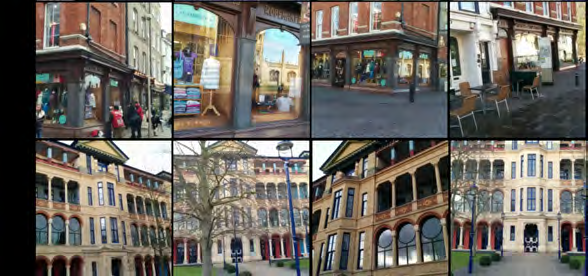
\includegraphics[width=\textwidth]{pics/Chapter2/cambridge.png}
    \caption{Minh họa tập dữ liệu Cambridge Landmarks \cite{kendall2016posenet}}
\end{figure}
\subsubsection*{Niantic Map-free Relocalization Dataset}
Tập dữ liệu Niantic Map-free Relocalization \cite{arnold2022mapfree} là một tập dữ liệu được thu thập chủ yếu để giúp ích cho phương pháp định vị Map-free \cite{arnold2022mapfree}. Tập dữ liệu bao gồm 655 cảnh bên ngoài với mỗi cảnh sẽ chứa một "địa điểm đáng chú ý" như một pho tượng, cổng, bảng hiệu,... sao cho địa điểm đó phải được xác định rõ trong một bức ảnh. Các cảnh được chia ra thành 460 cảnh phục vụ cho tác vụ huấn luyện, 65 cảnh phục vụ cho tác vụ kiểm tra quy trình huấn luyện và 130 cảnh phục vụ cho quá trình kiểm thử. Mỗi ảnh trong tập huấn luyện đều được gắn kèm vị trí tuyệt đối. Với tập kiểm thử và kiểm tra quy trình, mỗi cảnh sẽ được kèm theo một ảnh đại diện cũng như vị trí tuyệt đối tại cảnh. Ngoài ra, ma trận tham số nội tại của máy ảnh cũng được gắn kèm theo mỗi ảnh trong tập dữ liệu.
\begin{figure}[H]
    \centering
    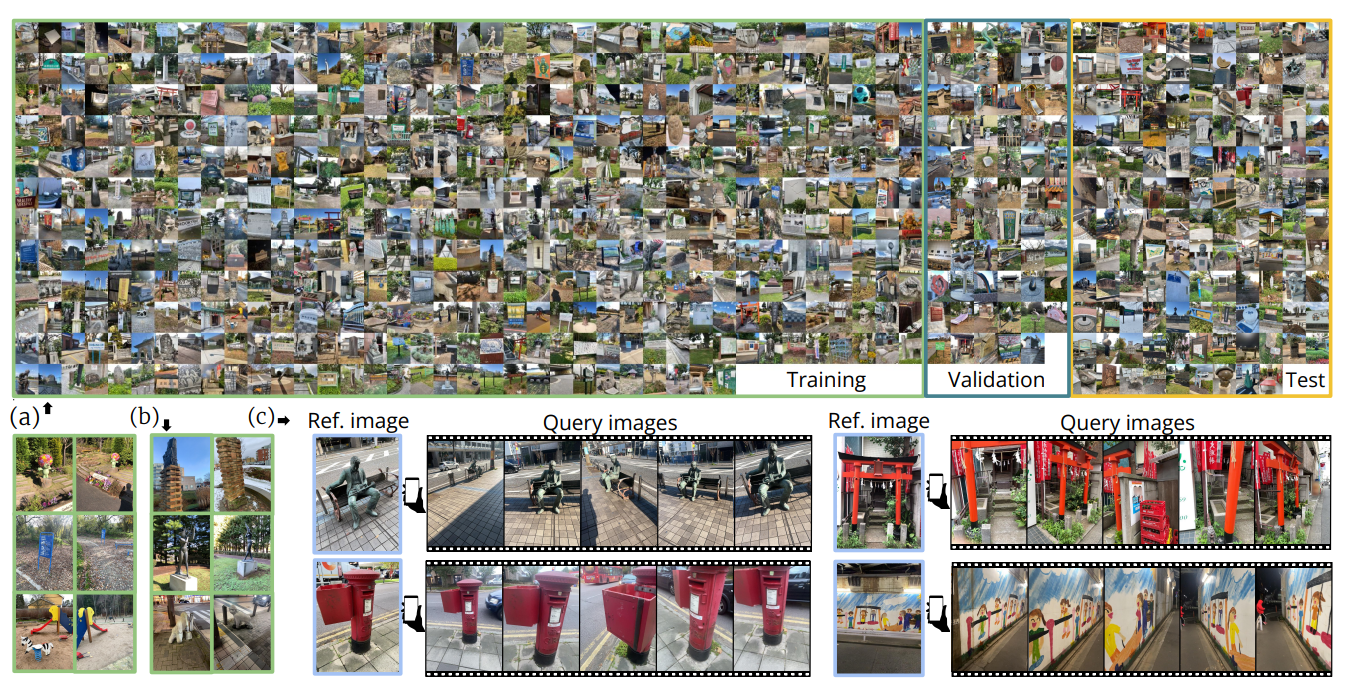
\includegraphics[width=\textwidth]{pics/Chapter2/niantic.png}
    \caption{Minh họa tập dữ liệu Niantic Map-free Relocalization \cite{arnold2022mapfree}}
\end{figure}
\subsection{Tập dữ liệu thành thị}
\subsubsection*{Aachen Day-Night}
Tập dữ liệu Aachen Day-Night \cite{Sattler2012ImageRF} bao gồm 14.607 ảnh được chụp với nhiều máy ảnh khác nhau bao phủ cả thành phố Aachen thuộc quốc gia Đức. Các ảnh dữ liệu được chụp ở nhiểu thời điểm trong ngày và trong năm, cụ thể là khoảng thời gian trong 2 năm. Hệ quả mang lại là tập dữ liệu bao phủ nhiều điều kiện ngoại cảnh như thời tiết, ánh sáng cũng như sự thay đổi của công trình kiến trúc trong khu vực.
\begin{figure}[H]
    \centering
    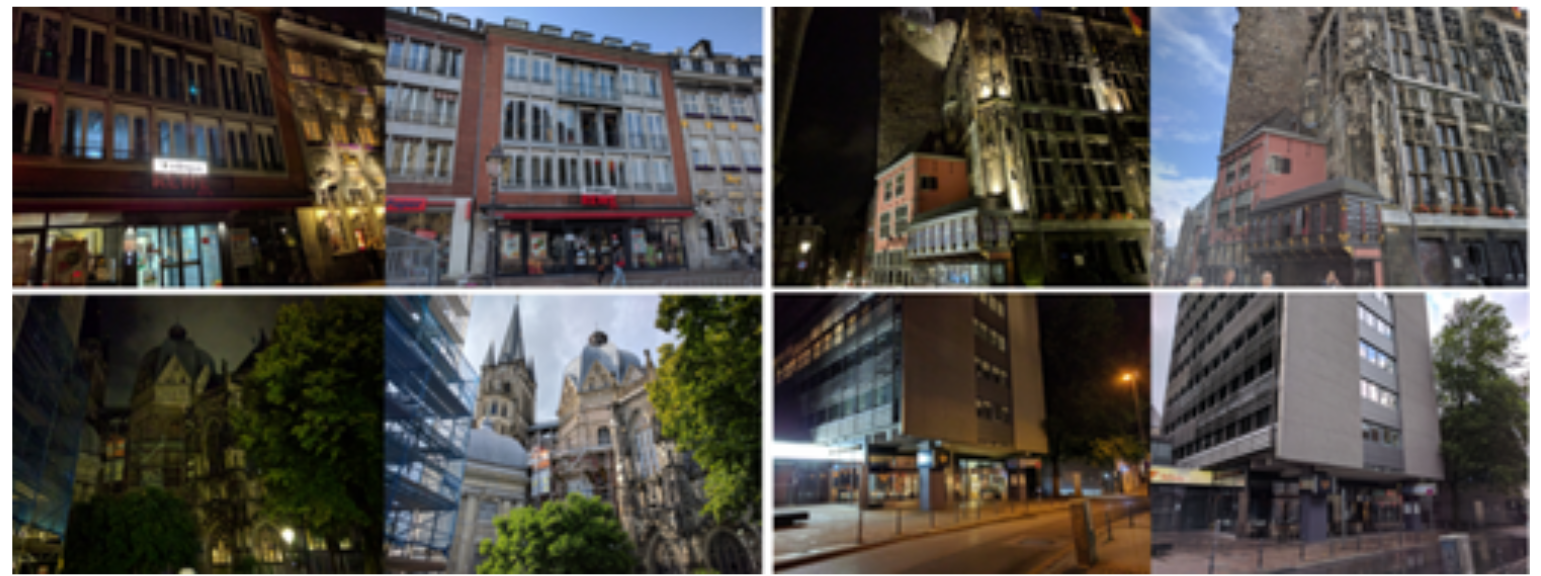
\includegraphics[width=\textwidth]{pics/Chapter2/aachen.png}
    \caption{Minh họa tập dữ liệu Aachen Day-Night \cite{Sattler2012ImageRF}}
\end{figure}
\subsubsection*{Pittsburgh 250k}
Tập dữ liệu Pittsburgh 250k \cite{6618963} là một tập dữ liệu tương đối rộng bao phủ thành phố Pittsburgh của Mỹ. Đây là một tập dữ liệu tương đối phổ biến trong thị giác máy tính, cụ thể là ở tác vụ nhận điện địa điểm trực quan, truy xuất ảnh và định vị trực quan.

\subsubsection*{GSV-Cities}
Tập dữ liệu GSV-Cities \cite{Ali_bey_2022} bao phủ một vùng địa lý cực kỳ rộng lớn với hơn 40 thành phố xuyên lục địa trong khoảng thời gian 14 năm liên tục. GSV-Cities chứa khoảng hơn 530.000 ảnh - khoảng hơn 62.000 vị trí. Mỗi vị trí sẽ có khoảng từ 4 đến 20 ảnh. Đồng thời mỗi vị trí sẽ cách nhau một khoảng ít nhất 100m.
\begin{figure}[H]
    \centering
    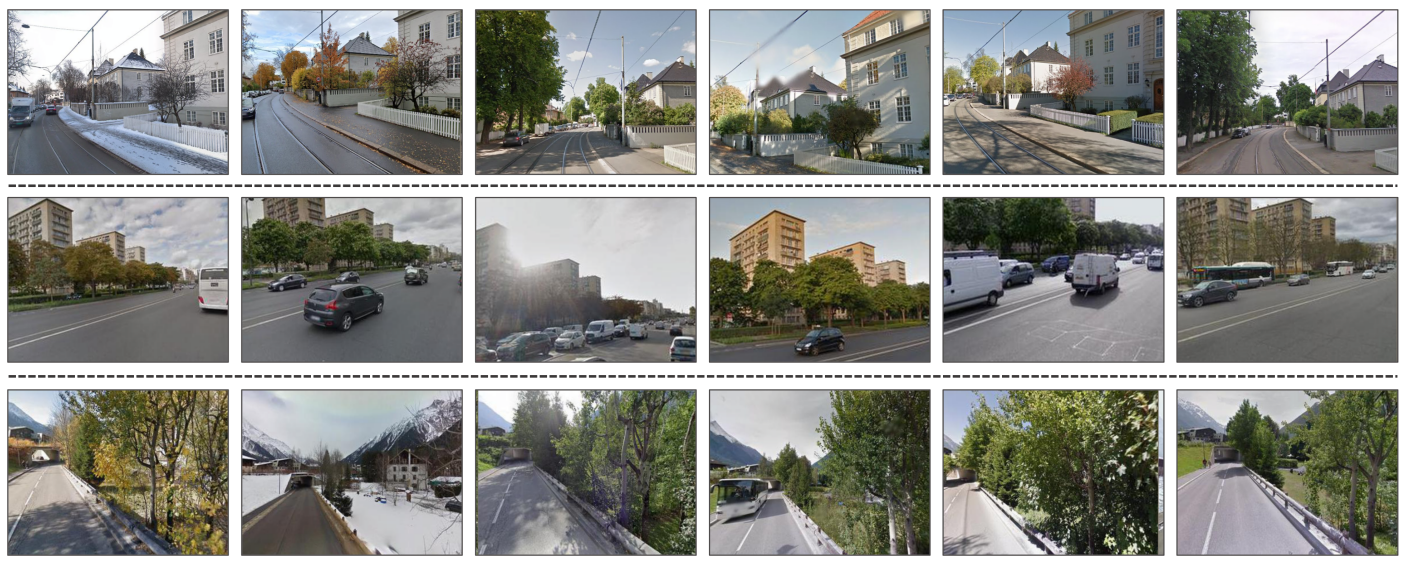
\includegraphics[width=\textwidth]{pics/Chapter2/gsv.png}
    \caption{Minh họa tập dữ liệu GSV-Cities \cite{Ali_bey_2022}}
\end{figure}

\subsubsection*{SF-XL}
Tập dữ liệu San Francisco Extra Large (SF-XL) \cite{berton2022rethinking} được tạo nên từ 3.43 triệu ảnh 360 độ thu thập từ kho ảnh Google Streetview. Các ảnh này sau đó được cắt ra thành 41.2 triệu ảnh. Mỗi ảnh cắt ra đều được gắn nhãn 6DoF (bao gồm cả GPS). Dữ liệu được thu thập từ năm 2009 đến năm 2021, dẫn đến việc tập dữ liệu bao phủ nhiều điều kiện ngoại cảnh như thời tiết, ánh sáng cũng như sự thay đổi của công trình kiến trúc trong khu vực.
\begin{figure}[H]
    \centering
    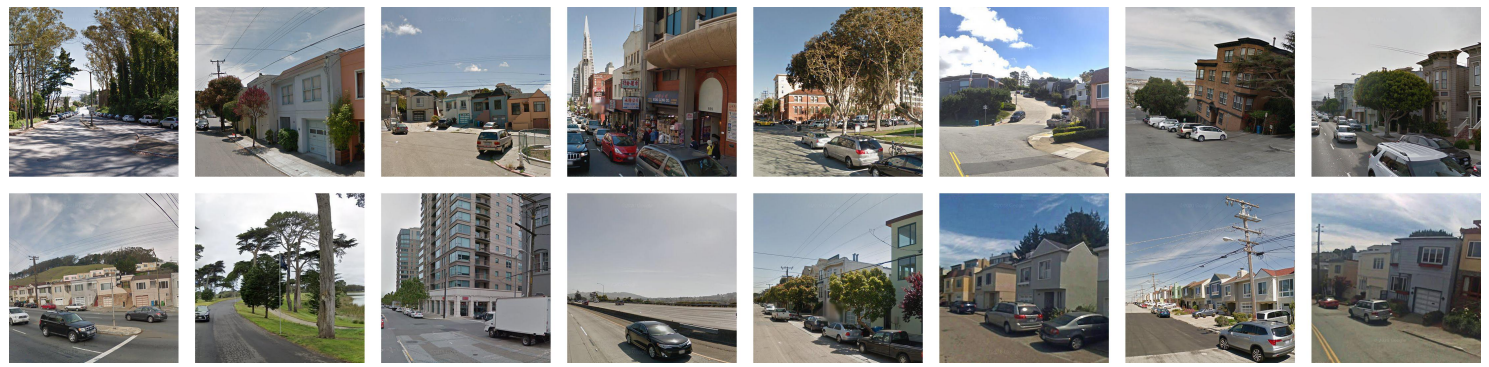
\includegraphics[width=\textwidth]{pics/Chapter2/sfxl.png}
    \caption{Minh họa tập dữ liệu San Francisco Extra Large \cite{berton2022rethinking}}
\end{figure}

\section{Mô hình MixVPR}
\subsection*{Mô tả quá trình thực nghiệm}
\subsection*{Kết quả thực nghiệm}
\subsection*{Nhận xét}


\section{Mô hình Map-free Relocalization}
\subsection*{Mô tả quá trình thực nghiệm}
\subsection*{Kết quả thực nghiệm}
\subsection*{Nhận xét}

\section{Hướng phát triển}

\section{Kết luận}